% Options for packages loaded elsewhere
\PassOptionsToPackage{unicode}{hyperref}
\PassOptionsToPackage{hyphens}{url}
\PassOptionsToPackage{dvipsnames,svgnames,x11names}{xcolor}
%
\documentclass[
  10pt,
  a4paper,
  DIV=11,
  numbers=noendperiod]{scrartcl}

\usepackage{amsmath,amssymb}
\usepackage{iftex}
\ifPDFTeX
  \usepackage[T1]{fontenc}
  \usepackage[utf8]{inputenc}
  \usepackage{textcomp} % provide euro and other symbols
\else % if luatex or xetex
  \usepackage{unicode-math}
  \defaultfontfeatures{Scale=MatchLowercase}
  \defaultfontfeatures[\rmfamily]{Ligatures=TeX,Scale=1}
\fi
\usepackage{lmodern}
\ifPDFTeX\else  
    % xetex/luatex font selection
\fi
% Use upquote if available, for straight quotes in verbatim environments
\IfFileExists{upquote.sty}{\usepackage{upquote}}{}
\IfFileExists{microtype.sty}{% use microtype if available
  \usepackage[]{microtype}
  \UseMicrotypeSet[protrusion]{basicmath} % disable protrusion for tt fonts
}{}
\makeatletter
\@ifundefined{KOMAClassName}{% if non-KOMA class
  \IfFileExists{parskip.sty}{%
    \usepackage{parskip}
  }{% else
    \setlength{\parindent}{0pt}
    \setlength{\parskip}{6pt plus 2pt minus 1pt}}
}{% if KOMA class
  \KOMAoptions{parskip=half}}
\makeatother
\usepackage{xcolor}
\setlength{\emergencystretch}{3em} % prevent overfull lines
\setcounter{secnumdepth}{5}
% Make \paragraph and \subparagraph free-standing
\makeatletter
\ifx\paragraph\undefined\else
  \let\oldparagraph\paragraph
  \renewcommand{\paragraph}{
    \@ifstar
      \xxxParagraphStar
      \xxxParagraphNoStar
  }
  \newcommand{\xxxParagraphStar}[1]{\oldparagraph*{#1}\mbox{}}
  \newcommand{\xxxParagraphNoStar}[1]{\oldparagraph{#1}\mbox{}}
\fi
\ifx\subparagraph\undefined\else
  \let\oldsubparagraph\subparagraph
  \renewcommand{\subparagraph}{
    \@ifstar
      \xxxSubParagraphStar
      \xxxSubParagraphNoStar
  }
  \newcommand{\xxxSubParagraphStar}[1]{\oldsubparagraph*{#1}\mbox{}}
  \newcommand{\xxxSubParagraphNoStar}[1]{\oldsubparagraph{#1}\mbox{}}
\fi
\makeatother


\providecommand{\tightlist}{%
  \setlength{\itemsep}{0pt}\setlength{\parskip}{0pt}}\usepackage{longtable,booktabs,array}
\usepackage{calc} % for calculating minipage widths
% Correct order of tables after \paragraph or \subparagraph
\usepackage{etoolbox}
\makeatletter
\patchcmd\longtable{\par}{\if@noskipsec\mbox{}\fi\par}{}{}
\makeatother
% Allow footnotes in longtable head/foot
\IfFileExists{footnotehyper.sty}{\usepackage{footnotehyper}}{\usepackage{footnote}}
\makesavenoteenv{longtable}
\usepackage{graphicx}
\makeatletter
\newsavebox\pandoc@box
\newcommand*\pandocbounded[1]{% scales image to fit in text height/width
  \sbox\pandoc@box{#1}%
  \Gscale@div\@tempa{\textheight}{\dimexpr\ht\pandoc@box+\dp\pandoc@box\relax}%
  \Gscale@div\@tempb{\linewidth}{\wd\pandoc@box}%
  \ifdim\@tempb\p@<\@tempa\p@\let\@tempa\@tempb\fi% select the smaller of both
  \ifdim\@tempa\p@<\p@\scalebox{\@tempa}{\usebox\pandoc@box}%
  \else\usebox{\pandoc@box}%
  \fi%
}
% Set default figure placement to htbp
\def\fps@figure{htbp}
\makeatother

\usepackage{tikz}
\usepackage{xspace}
\usepackage{adjustbox}
\usetikzlibrary{positioning,arrows,arrows.meta,shapes.geometric,fit,calc,backgrounds}
% Generated alongside the figure - keeps the numbers in the prose from
% drifting away from the pipeline sources. See figures/make_pipeline_uml.py.
% !! GENERATED FILE - do not edit. See paper/figures/make_pipeline_uml.py
\newcommand{\PanelSize}{3\xspace}
\newcommand{\NumDimensions}{5\xspace}
\newcommand{\NumMultiDimensions}{4\xspace}
\newcommand{\NumCategories}{54\xspace}
\newcommand{\NumStages}{23\xspace}
\newcommand{\NumTokenStages}{10\xspace}
\newcommand{\PinnedModel}{\texttt{mistral-medium-3.5-128b}\xspace}
\newcommand{\DimensionList}{\texttt{research\_position}, \texttt{software\_lifecycle}, \texttt{software\_type}, \texttt{techstack}, \texttt{evaluation}\xspace}

\KOMAoption{captions}{tableheading}
\makeatletter
\@ifpackageloaded{caption}{}{\usepackage{caption}}
\AtBeginDocument{%
\ifdefined\contentsname
  \renewcommand*\contentsname{Table of contents}
\else
  \newcommand\contentsname{Table of contents}
\fi
\ifdefined\listfigurename
  \renewcommand*\listfigurename{List of Figures}
\else
  \newcommand\listfigurename{List of Figures}
\fi
\ifdefined\listtablename
  \renewcommand*\listtablename{List of Tables}
\else
  \newcommand\listtablename{List of Tables}
\fi
\ifdefined\figurename
  \renewcommand*\figurename{Figure}
\else
  \newcommand\figurename{Figure}
\fi
\ifdefined\tablename
  \renewcommand*\tablename{Table}
\else
  \newcommand\tablename{Table}
\fi
}
\@ifpackageloaded{float}{}{\usepackage{float}}
\floatstyle{ruled}
\@ifundefined{c@chapter}{\newfloat{codelisting}{h}{lop}}{\newfloat{codelisting}{h}{lop}[chapter]}
\floatname{codelisting}{Listing}
\newcommand*\listoflistings{\listof{codelisting}{List of Listings}}
\makeatother
\makeatletter
\makeatother
\makeatletter
\@ifpackageloaded{caption}{}{\usepackage{caption}}
\@ifpackageloaded{subcaption}{}{\usepackage{subcaption}}
\makeatother

\usepackage{bookmark}

\IfFileExists{xurl.sty}{\usepackage{xurl}}{} % add URL line breaks if available
\urlstyle{same} % disable monospaced font for URLs
\hypersetup{
  pdftitle={What Research Software do Computer Scientists Build? A Typology and Corpus Study of the Lecture Notes in Informatics},
  pdfauthor={Julian Dehne},
  pdfkeywords={research software engineering, software
typology, empirical software engineering, LLM-assisted
annotation, corpus study},
  colorlinks=true,
  linkcolor={blue},
  filecolor={Maroon},
  citecolor={Blue},
  urlcolor={Blue},
  pdfcreator={LaTeX via pandoc}}


\title{What Research Software do Computer Scientists Build? A Typology
and Corpus Study of the Lecture Notes in Informatics}
\author{Julian Dehne}
\date{2026-08-05}

\begin{document}
\maketitle
\begin{abstract}
Research software engineering has concentrated on the STEM domains that
\emph{consume} research software and has largely overlooked software
engineering itself as a discipline that \emph{produces} it. We derive an
empirical typology of computer-science research software from the
German-language \emph{Lecture Notes in Informatics} corpus of roughly
14,000 papers. Each paper is first gated on whether it reports research
software at all and then classified along five dimensions: position in
the research process, software-lifecycle phase, type of software,
techstack, and mode of evaluation. The scheme is bootstrapped by a large
language model, narrowed by human review, and validated by two coders
against a goldstandard. The full corpus is then annotated by a panel of
the three best-performing models, whose answers are merged by majority
vote. We report how research software is distributed across the
typology, where the reported lifecycle is thin, and how far model
agreement can be trusted. The typology, prompts, and pipeline are
released for replication.
\end{abstract}


\section{Introduction}\label{introduction}

Research software engineering (RSE) research has so far described the
software of the disciplines that \emph{use} computation --- physics, the
life sciences, the digital humanities --- and has treated computer
science mostly as the supplier of methods rather than as a producing
discipline in its own right. That is an odd gap: computer science is the
field in which software is most tightly bound to the research claim
itself, and where a prototype is often not the instrument of the result
but the result.

This paper asks what that software actually looks like. We take the
German-language \emph{Lecture Notes in Informatics} (LNI) series as a
large, discipline-spanning and largely unstudied corpus, and derive an
empirical typology of the research software reported in it.

\textbf{Contributions.}

\begin{itemize}
\tightlist
\item
  An empirical typology of computer-science research software with
  \NumDimensions dimensions and \NumCategories categories, grounded in a
  corpus rather than postulated.
\item
  A human goldstandard of LNI papers, double-coded, with intercoder
  reliability reported per dimension.
\item
  A reproducible LLM annotation pipeline in which model choice is an
  \emph{empirical} decision and the corpus is labelled by a
  majority-voting panel of \PanelSize models rather than by one model.
\item
  TODO --- the substantive findings, once the full run is complete.
\end{itemize}

\section{Background and Related Work}\label{background-and-related-work}

TODO. Three strands: (i) definitions and taxonomies of research
software; (ii) corpus and mining studies of software mentioned in
papers; (iii) LLMs as annotators in empirical software engineering, and
the reliability evidence for using them in place of, or alongside, human
coders.

\section{Research Questions}\label{research-questions}

\textbf{RQ1.} How much of the LNI corpus reports research software at
all?

\textbf{RQ2.} How is that software distributed across the
\NumDimensions typology dimensions --- in particular, is it reported as
a \emph{result} of the research process or as \emph{machinery} used
within it?

\textbf{RQ3.} Which lifecycle phases are systematically under-reported?

\textbf{RQ4.} How reliable is a majority-voting LLM panel as a
substitute for human coding on this task, per dimension?

\section{Study Design}\label{study-design}

The study runs as a single reproducible pipeline; Figure
\ref{fig:pipeline} shows its process flow as a UML activity diagram. The
figure is \emph{generated from the pipeline sources}, so it cannot
describe a step the code no longer has.

% !! GENERATED FILE - do not edit. See paper/figures/make_pipeline_uml.py
\begin{figure}[tbp]
  \centering
  \adjustbox{max width=\linewidth, max totalheight=0.86\textheight}{%
  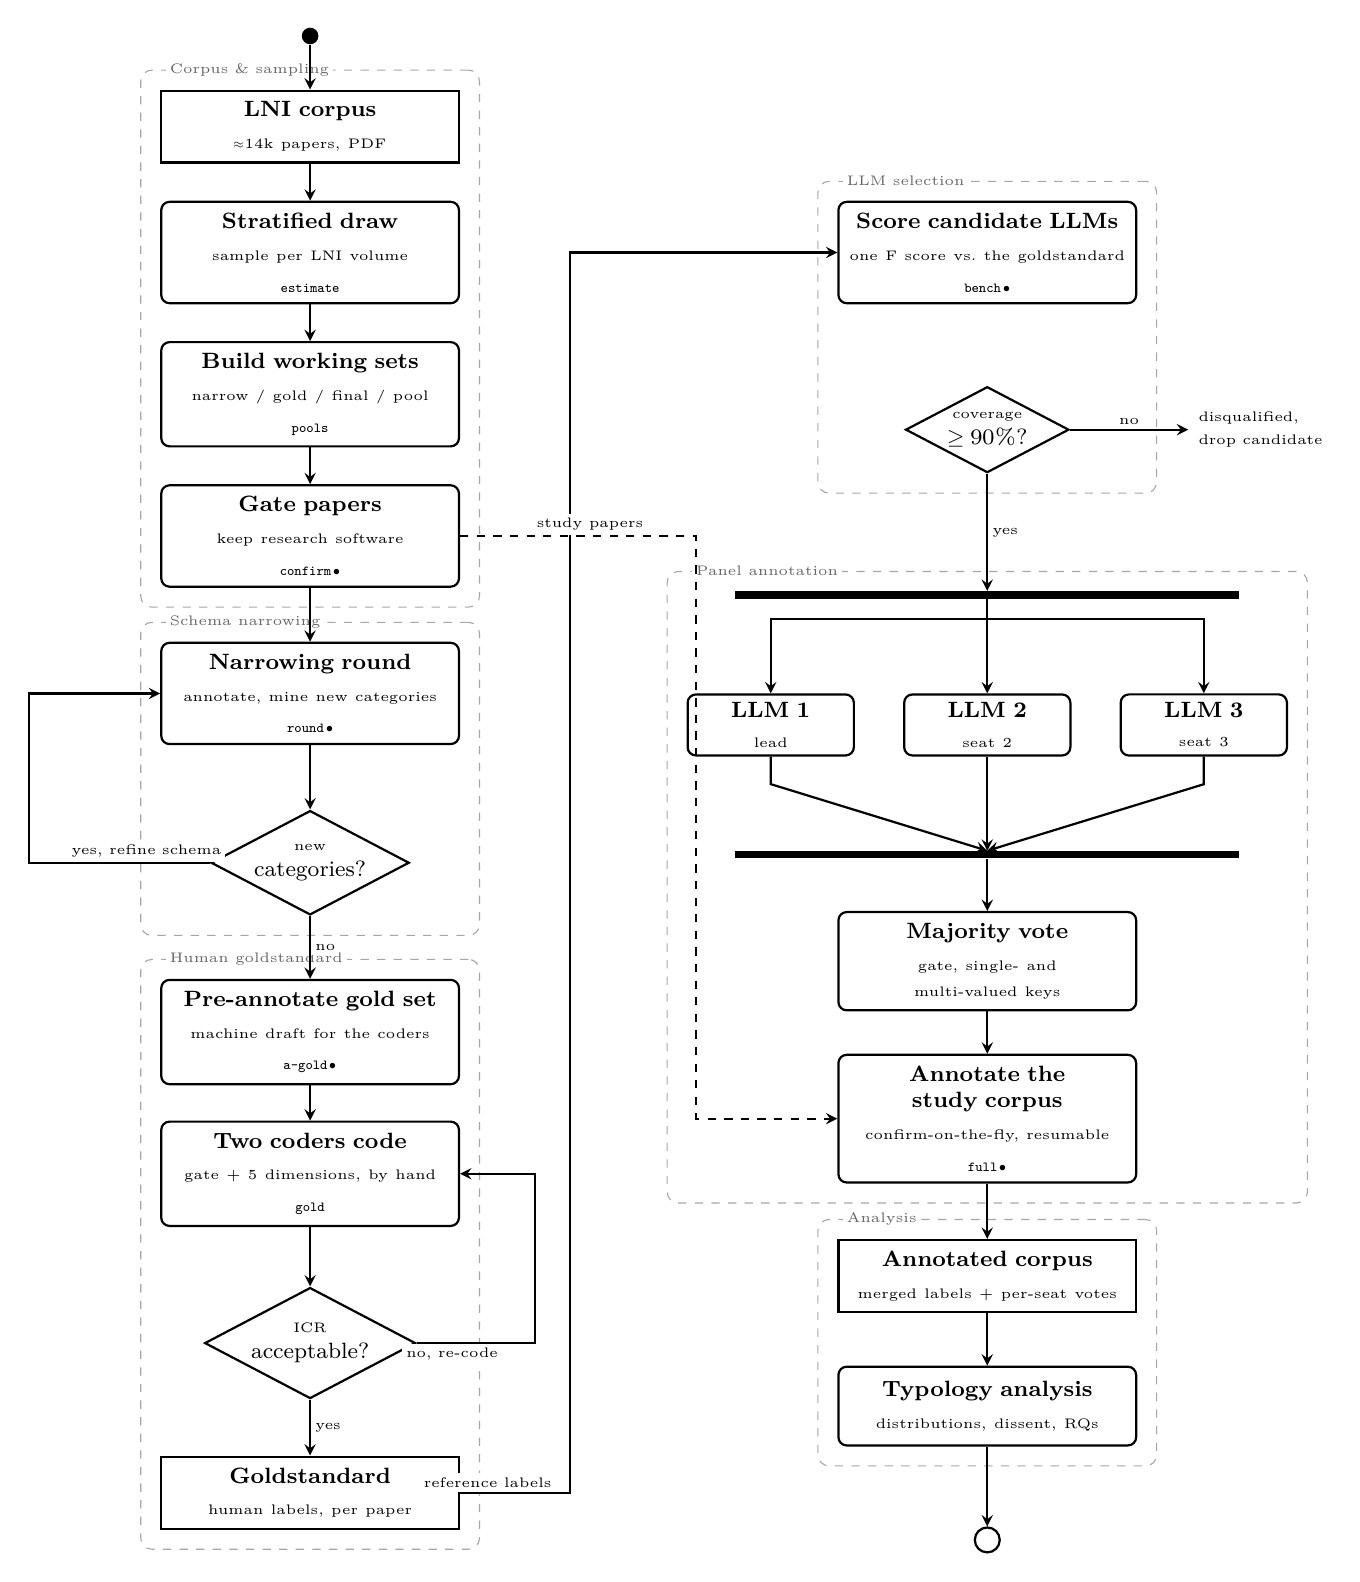
\begin{tikzpicture}[
    font=\footnotesize,
    action/.style={rounded corners=3pt, draw, thick, fill=white, text width=3.5cm, align=center, inner sep=4pt, minimum height=1cm},
    objectnode/.style={draw, thick, fill=white, text width=3.5cm, align=center, inner sep=4pt, minimum height=0.9cm},
    decision/.style={diamond, draw, thick, fill=white, aspect=1.9, align=center, inner sep=1pt},
    seat/.style={rounded corners=3pt, draw, thick, fill=white, align=center, text width=1.9cm, inner sep=3pt},
    synchbar/.style={fill=black, minimum width=6.4cm, minimum height=2.6pt, inner sep=0pt},
    initial node/.style={circle, fill=black, minimum size=6pt, inner sep=0pt},
    final node/.style={circle, draw, thick, fill=white, minimum size=9pt, inner sep=0pt, path picture={\fill (path picture bounding box.center) circle (2.2pt);}},
    flow/.style={-stealth, thick},
    elabel/.style={inner sep=1.5pt, fill=white},
    partition/.style={draw=black!35, dashed, rounded corners=4pt, inner sep=7pt},
    partlabel/.style={anchor=west, text=black!60, fill=white, inner sep=1.5pt},
  ]
  \node[initial node] (start) at (0.00,0.00) {};
  \node[objectnode] (corpus) at (0.00,-1.15) {\textbf{LNI corpus}\\[2pt]{\tiny $\approx$14k papers, PDF}};
  \node[action] (draw) at (0.00,-2.75) {\textbf{Stratified draw}\\[2pt]{\tiny sample per LNI volume}\\[2pt]{\tiny \texttt{estimate}}};
  \node[action] (pools) at (0.00,-4.55) {\textbf{Build working sets}\\[2pt]{\tiny narrow / gold / final / pool}\\[2pt]{\tiny \texttt{pools}}};
  \node[action] (conf) at (0.00,-6.35) {\textbf{Gate papers}\\[2pt]{\tiny keep research software}\\[2pt]{\tiny \texttt{confirm}\,$\bullet$}};
  \node[action] (round) at (0.00,-8.35) {\textbf{Narrowing round}\\[2pt]{\tiny annotate, mine new categories}\\[2pt]{\tiny \texttt{round}\,$\bullet$}};
  \node[decision] (dcat) at (0.00,-10.50) {\tiny new\\categories?};
  \node[action] (agold) at (0.00,-12.65) {\textbf{Pre-annotate gold set}\\[2pt]{\tiny machine draft for the coders}\\[2pt]{\tiny \texttt{a-gold}\,$\bullet$}};
  \node[action] (gold) at (0.00,-14.45) {\textbf{Two coders code}\\[2pt]{\tiny gate + 5 dimensions, by hand}\\[2pt]{\tiny \texttt{gold}}};
  \node[decision] (dicr) at (0.00,-16.60) {\tiny ICR\\acceptable?};
  \node[objectnode] (goldstd) at (0.00,-18.50) {\textbf{Goldstandard}\\[2pt]{\tiny human labels, per paper}};
  \node[action] (bench) at (8.60,-2.75) {\textbf{Score candidate LLMs}\\[2pt]{\tiny one F score vs.\ the goldstandard}\\[2pt]{\tiny \texttt{bench}\,$\bullet$}};
  \node[decision] (dcov) at (8.60,-5.00) {\tiny coverage\\$\geq 90\%$?};
  \node[synchbar] (fork) at (8.60,-7.10) {};
  \node[synchbar] (join) at (8.60,-10.40) {};
  \node[action] (vote) at (8.60,-11.75) {\textbf{Majority vote}\\[2pt]{\tiny gate, single- and multi-valued keys}};
  \node[action] (full) at (8.60,-13.75) {\textbf{Annotate the study corpus}\\[2pt]{\tiny confirm-on-the-fly, resumable}\\[2pt]{\tiny \texttt{full}\,$\bullet$}};
  \node[objectnode] (dataset) at (8.60,-15.75) {\textbf{Annotated corpus}\\[2pt]{\tiny merged labels + per-seat votes}};
  \node[action] (analyse) at (8.60,-17.40) {\textbf{Typology analysis}\\[2pt]{\tiny distributions, dissent, RQs}};
  \node[final node] (end) at (8.60,-19.10) {};
  \node[seat] (seat0) at (5.85,-8.75) {\textbf{LLM 1}\\[1pt]{\tiny lead}};
  \node[seat] (seat1) at (8.60,-8.75) {\textbf{LLM 2}\\[1pt]{\tiny seat 2}};
  \node[seat] (seat2) at (11.35,-8.75) {\textbf{LLM 3}\\[1pt]{\tiny seat 3}};
  \draw[flow] (start) -- (corpus);
  \draw[flow] (corpus) -- (draw);
  \draw[flow] (draw) -- (pools);
  \draw[flow] (pools) -- (conf);
  \draw[flow] (conf) -- (round);
  \draw[flow] (round) -- (dcat);
  \draw[flow] (dcat) -- node[elabel,right] {\tiny no} (agold);
  \draw[flow] (agold) -- (gold);
  \draw[flow] (gold) -- (dicr);
  \draw[flow] (dicr) -- node[elabel,right] {\tiny yes} (goldstd);
  \draw[flow] (dcov) -- node[elabel,right] {\tiny yes} (fork);
  \draw[flow] (join) -- (vote);
  \draw[flow] (vote) -- (full);
  \draw[flow] (full) -- (dataset);
  \draw[flow] (dataset) -- (analyse);
  \draw[flow] (analyse) -- (end);
  \draw[flow] (fork.south) -- ++(0,-0.25) -| (seat0.north);
  \draw[flow] (seat0.south) |- ++(0,-0.35) -- (join.north);
  \draw[flow] (fork.south) -- ++(0,-0.25) -| (seat1.north);
  \draw[flow] (seat1.south) |- ++(0,-0.35) -- (join.north);
  \draw[flow] (fork.south) -- ++(0,-0.25) -| (seat2.north);
  \draw[flow] (seat2.south) |- ++(0,-0.35) -- (join.north);
  \draw[flow] (dcat.west) -- node[elabel,above,pos=0.35] {\tiny yes, refine schema} ++(-2.3,0) |- (round.west);
  \draw[flow] (dicr.east) -- node[elabel,below,pos=0.3] {\tiny no, re-code} ++(1.5,0) |- (gold.east);
  \draw[flow] (goldstd.east) -- node[elabel,above,pos=0.25] {\tiny reference labels} ++(1.4,0) |- (bench.west);
  \draw[flow] (dcov.east) -- node[elabel,above] {\tiny no} ++(1.5,0) node[right,align=left] {\tiny disqualified,\\[-1pt]\tiny drop candidate};
  \draw[flow,dashed] (conf.east) -- node[elabel,above,pos=0.55] {\tiny study papers} ++(3.0,0) |- (full.west);
  \begin{scope}[on background layer]
    \node[partition,fit=(corpus) (draw) (pools) (conf)] (p0) {};
    \node[partlabel] at ($(p0.north west)+(9pt,0)$) {\tiny Corpus \& sampling};
    \node[partition,fit=(round) (dcat)] (p1) {};
    \node[partlabel] at ($(p1.north west)+(9pt,0)$) {\tiny Schema narrowing};
    \node[partition,fit=(agold) (gold) (dicr) (goldstd)] (p2) {};
    \node[partlabel] at ($(p2.north west)+(9pt,0)$) {\tiny Human goldstandard};
    \node[partition,fit=(bench) (dcov)] (p3) {};
    \node[partlabel] at ($(p3.north west)+(9pt,0)$) {\tiny LLM selection};
    \node[partition,fit=(fork) (seat0) (seat1) (seat2) (join) (vote) (full)] (p4) {};
    \node[partlabel] at ($(p4.north west)+(9pt,0)$) {\tiny Panel annotation};
    \node[partition,fit=(dataset) (analyse)] (p5) {};
    \node[partlabel] at ($(p5.north west)+(9pt,0)$) {\tiny Analysis};
  \end{scope}
  \end{tikzpicture}%
  }
  \caption{Process flow of the annotation pipeline as a UML activity diagram. Rounded boxes are actions, the monospaced key is the pipeline step that runs them (\texttt{run\_pipeline.cmd <step>}); $\bullet$ marks the 10 steps that spend LLM calls. Papers pass the research-software gate before they are typed along 5 dimensions (\texttt{research\_position}, \texttt{software\_lifecycle}, \texttt{software\_type}, \texttt{techstack}, \texttt{evaluation}) holding 54 categories in total. The fork/join is the annotation panel: the 3 best-scoring models of the selection step classify every paper independently and their answers are merged by majority vote, with the highest-scoring model breaking ties. Generated from the pipeline sources by \texttt{paper/figures/make\_pipeline\_uml.py}.}
  \label{fig:pipeline}
\end{figure}


\subsection{Corpus and sampling}\label{corpus-and-sampling}

The LNI series comprises roughly 14,000 papers across conference and
workshop volumes. Working sets are drawn by a stratified sample per
volume, so no single venue or year dominates either the schema-narrowing
rounds or the goldstandard.

\subsection{The typology}\label{the-typology}

Papers are first passed through a gate --- does this paper report
research software? --- and only accepted papers are typed. The typology
has \NumDimensions dimensions (\DimensionList), of which
\NumMultiDimensions admit more than one value per paper, and
\NumCategories categories in total. The initial scheme was bootstrapped
by an LLM over a narrowing set and then reduced by human review over
successive rounds until no round proposed a category that survived;
categories that were retired are marked deprecated rather than deleted,
so earlier annotations remain interpretable.

\subsection{Human goldstandard}\label{human-goldstandard}

A goldstandard set is pre-annotated by the model to give the coders a
draft, and then coded by two humans independently along the gate and all
\NumDimensions dimensions. Intercoder reliability is computed per
dimension; where it is not acceptable the schema descriptions are
sharpened and the affected papers are re-coded. TODO --- report the
final ICR values and the number of re-coding rounds.

\subsection{LLM annotation panel}\label{llm-annotation-panel}

Which models annotate the corpus is decided empirically rather than by
preference. Every candidate model re-annotates the whole goldstandard
and is scored against the human labels with a single combined F score
--- macro-F1 on the gate, exact match and micro-F1 on the typology
dimensions --- with no held-out split, since nothing is trained.
Candidates that fail to return parseable answers for at least 90 \% of
the papers are disqualified outright. The \PanelSize best-scoring
survivors form the annotation panel; the highest scorer is the lead and
breaks ties.

The corpus is then annotated by all \PanelSize panel members
independently and their answers are merged by majority vote: the gate is
decided by a majority of the votes actually cast --- a model that errors
abstains rather than voting ``no'' --- single-valued dimensions take the
modal category, and each key of a multi-valued dimension is kept when it
appears in a majority of the cast votes. Every merged row carries the
individual votes and a dissent marker, and the raw per-model answers are
kept, so any claim in Section 5 can be recomputed against a single model
or against the panel's disagreement rather than only against the merged
label.

\subsection{Analysis}\label{analysis}

TODO. Distributions per dimension, co-occurrence between dimensions,
panel dissent as an uncertainty measure, and the comparison of panel
labels against the human goldstandard that answers RQ4.

\section{Results}\label{results}

TODO --- awaiting the full annotation run.

\section{Discussion}\label{discussion}

TODO.

\section{Threats to Validity}\label{threats-to-validity}

\textbf{Construct validity.} The typology is derived from what papers
\emph{report}, not from what their authors built; software that exists
but is not described is invisible to the study by construction.

\textbf{Internal validity.} The goldstandard PDFs available locally lean
towards accepted papers, which skews the measurement of gate performance
--- typology scores are unaffected. Model selection uses one score over
the whole goldstandard with nothing held out; the panel of
\PanelSize mitigates, but does not remove, the risk that a seat was won
by a narrow margin.

\textbf{External validity.} LNI is a German-language, largely national
venue series. Findings transfer to comparable community series with care
and not automatically to international top-tier venues.

\textbf{Reliability.} The pipeline, prompts, category schema and
analysis code are released; LLM answers are non-deterministic, so exact
per-paper replication is not guaranteed even at a fixed temperature. The
per-model answers are published alongside the merged labels to make the
residual variance inspectable.

\section{Conclusion}\label{conclusion}

TODO.

\section{Declarations}\label{declarations}

\textbf{Data availability.} TODO --- link the replication package
(schema, prompts, goldstandard coding, merged annotations, per-model
votes).

\textbf{Funding and competing interests.} TODO.




\end{document}
